\chapter{Systematic Exploration of Power-Aware Scenarios for IEEE 802.11ac WLAN Systems}
\label{dsd}

\begin{center}
Nikolaos Zompakis, Iason Filippopoulos, Per Gunnar Kjeldsberg, Francky Catthoor and Dimitrios Soudris
\\
17th Euromicro Conference on Digital System Design (DSD) 
\\
IEEE
\\
pages 28–35, 2014
\end{center}
\afterpage{\null\newpage}
\newpage

\vspace*{\fill}
\phantomsection
\section*{\hspace*{\fill} Abstract \hspace*{\fill}}
\addcontentsline{toc}{section}{Abstract}
This work explores the power management options for a transmitting wireless system using system scenarios. We exploit the variations in the communication channel and the protocol requirements during the lifetime of a transmission, in order to optimize energy usage. Both the transmission signal power and the memory subsystem are taken into consideration. Different system scenarios and the corresponding configurations capture the different resource requirements, which change dynamically during transmission. Signal power on the antenna and active memory banks are the two main platform parameters explored in this study and sufficiently detailed system models are presented for both. The trade-off between the accuracy of the generated system scenarios and the switching cost between them is analyzed. The exploration is performed for an increasing number of system scenarios, from 1 to 14, and the reported power gains are over 95\% and over 25\% on the signal power and the memory subsystems respectively.
\vspace*{\fill}
\afterpage{\null\newpage}
\newpage

\section{Introduction}

Modern wireless technology \cite{1} has opened new horizons in the means and ways that users communicate. Radio devices exist in a multitude of items such as cell phones, tablet computers and digital TVs. The different types of applications demand different types of communication standards. Modern 4G networks provide high quality of services (QoS) exploiting new innovative techniques, which combine smart transceivers and high performance receivers. This trend creates new challenges that the conventional radio equipment cannot cope with. Promising technologies, like Software Defined Radio (SDR) \cite{2}, attempt to integrate the rapidly changing wireless networks, merging existing and new communication standards into one platform. In this context, IEEE 802.11 wireless local area networks (WLANs) play an important role in fourth-generation wireless mobile communication systems \cite{3}. The development of WLANs has primarily been guided by legacy IEEE 802.11a/b/g devices. With the recent emergence of the IEEE 802.11n and the upcoming 802.11ac standards, WLANs are given the option to operate over wider channels that achieve higher transmission rates. IEEE 802.11ac supports very high bandwidth communication with a targeted data rate greater than 1 Gbps in the band below 6 GHz \cite{4}.
	
Meanwhile, wireless applications become more and more resource demanding, intending to provide better QoS. However, the majority of these applications are operating under the limitations of the mobile handsets. Thus, the design challenges include both the high performance requirements and the low power consumption constraints. New techniques that can efficiently exploit the energy resources are undoubtedly an imperative need, in order to extend the battery life. In this direction, the signal power and the memory system represent the main sources of power consumption on a mobile device. Signal power account at least for 50\% of the power consumption when a mobile device is on a standby mode, and even more during calls. The memory subsystem has also an important contribution due to the data intensive nature of the wireless applications. Both the transmit power requirements on the antennas and the data requirements on the memory change dynamically. Smart antennas optimize automatically their transmission and their reception pattern responding to the changes of the external environment. Flexible OFDM systems exploit the channel state information adjusting the transmit power and increasing the achieved data rate \cite{5}\cite{6}. At the same time the chosen coding and modulation scheme for data transmission affects the memory requirements. 
	
	The dynamic behavior outlined above results in unnecessarily high energy consumption if the system is statically designed to accommodate the worst-case behavior. This is avoided if a system scenario methodology is applied \cite{17}. At design time a number of cost-optimized scenarios are selected so that the system can be reconfigured at run-time according to the current dynamic situation. In the current study, we consider a wireless system where the transmit power and the activity of the memory is adapted to the running situation based on application constraints and channel conditions. The scope is to classify from a cost perspective the functionality of a transmission process exploiting the system scenario methodology. The first main contribution is the specification of the energy optimal configurations of a potential wireless system focusing on the energy consumption of both transmission signals and memories. The second key contribution is that we examine the trade-off between the accuracy of the extracted scenarios and their switching overhead, which is correlated with the system configuration cost. For our purpose, a state of the art communication protocol (802.11ac) is chosen with a large fluctuation on the supported communication characteristics.

This paper is organized as follows. Section II surveys related work and differentiation of the current work. Section III presents an overview of the system scenario principles. In Section IV the system models for the signal power and the memory are described, while the case study of this work is analyzed in Section V. Results for the case study are shown in Section VI. Finally, conclusions are drawn in Section VII.

\section{Related Work}

Transmission signal power adaptation is a key issue for energy-aware wireless devices. Several algorithms have been proposed for dynamic power management of the antenna signal. The critical point in all cases is the interference of the neighbor users. In a wireless system, the power allocation problem can be efficiently addressed by the water-filling algorithm \cite{7}. The scope of this algorithm is to manage, in an optimal way, the antenna signal transmission power of every user in a wireless system network. The target is to maximize the available capacity of the transmission channel. The main drawback of this approach is that the provided QoS is not taken into consideration. QoS has been successfully considered in a number of other studies. In \cite{8} authors attempt to minimize the whole system transmission power under fixed performance requirements for a given sets of user data rates. In \cite{9} an extension of the traditional water-filling technique, considering users queue-length constraints, is presented. In the context of a cognitive radio OFDM system, authors in \cite{10} propose optimal power loading schemes for a single user and extend their proposal for multiple users in \cite{11}. In \cite{12} optimal power control policies are presented focusing on fading channel at cognitive radio networks. These policies pay special attention to the interference influence. All the above solutions have the drawback that they presuppose a centralized control, which implies significant changes to the network infrastructure. A second important drawback is that they are characterized by high implementation complexity.

In the context of the current study we work towards overcoming these drawbacks. Regarding the first, we propose a distributed power adjustment approach, which can be applied at client-platform level. This approach exploits the signal power scaling range between the minimum required SNR (Signal to Noise Ratio) (based on the noise conditions and the required data rate) and the permissible signal power radiation (EMC, FCC Rules Dictate Antenna Use). The main contribution is focused on the second design obstacle, which is related with the implementation complexity cost. In respect to that we apply a scenario-based methodology which provides the required flexibility to cluster and classify the multi-operation conditions into system scenarios which are effectively detected and exploited at run-time. The key issue is that we examine the trade-offs between the switching and clustering overhead. A somewhat similar trade-off was presented in \cite{24}, but this is the first time that it is applied in a systematic way for a wireless application and especially for the specific characteristics of WLAN IEEE 802.11ac systems.

A comprehensive study on a low-power architecture specifically designed for software radio is presented in \cite{22}. The target wireless protocols explored are W-CDMA and 802.11a and the power consumption breakdown is analyzed for the whole system. In both cases the memory architecture are an important contributor to the overall energy consumption, exceeding 30\% for the worst case. In \cite{23} a power saving mechanism for high speed WLAN applications is presented. The authors propose a hierarchical memory design to reduce memory access operations and report a 30 to 40\% power dissipation reduction. This method is complementary to ours, because it reduces the number of memory accesses while we focus on optimizing the energy per access. Again, the main differentiation with the current work is the scenario exploration, which is viable by employing a platform that is reconfigurable during run-time.

The system scenario methodology has been described in \cite{13} and is presented in Section III. The system scenario concept was also outlined in \cite{15}, where the tasks are written using a combination of a hierarchical finite state machine (FSM) and a synchronous dataflow model (SDF). The disadvantage of this method is that the applications must be written using a limited model, which is a time consuming and error-prone operation. In \cite{16} authors propose a scenario-based framework for managing processor resources while achieving QoS on contemporary multi-core processors running media-streaming applications. In \cite{21} the efficiency of system scenarios for dynamic wireless applications is shown. The usage of system scenarios on the memory is presented in \cite{Fil12}. In this study, the main focus is on the dynamic management of both the signal power and the memory activity. Apart from the application of the system scenario methodology on an emerging wireless protocol, we perform a design exploration trade-off analysis. To be more specific, we examine the main trade–off between clustering overhead, which is correlated with how representative are the scenarios, and switching overhead, which represents the tuning cost of the platform.

\section{System Scenario Principles}

The system scenario methodology is a design approach for handling the complexity analysis of applications with multi-dimensional costs and strict constraints. The main challenges are the optimal application mapping on the platform and the efficient management of the platform resources. In particular, by classifying and clustering the possible system executions into system scenarios, a run-time resource manager can substantially reduce the average cost resulting from this execution compared to the conventional worst-case bounding approach, while still meeting all constraints.

	The aim of system scenarios is to capture the data dependent dynamic behavior inside a thread in order to better schedule a multi-thread application on a heterogeneous multi-processor architecture. \cite{14} presents a design methodology that provides a systematic way of detecting and exploiting system scenarios for streaming applications. A scenario is defined as the application behavior for a specific type of input data, i.e. a group of execution paths for that particular group of input data.

An important term in the scenario methodology is the Run-Time Situation (RTS). An RTS is a deterministic thread execution path with specific and fixed cost dimensions. RTSs are treated as execution units. The system scenario methodology comprises 5 individual steps as defined by \cite{17}:
\begin{enumerate}
\item 	Identification. The first step is to identify all possible RTSs. To achieve this, we identify and classify all RTS parameters. As a parameter, we can assume every variable affecting the state of the system from a functionality point of view.
\item Characterization. Each RTS can be characterized by a number of cost factors obtained from profiling the application on a platform or by using high-level cost estimators. The placement of the possible cost points of each RTS on the cost space leads to a Pareto curve. The Pareto curve contains all the potential exploitation points in the multi-dimensional exploration space.
\item Clustering. It defines the grouping of the individual execution situations into system scenarios. The clustering process introduces inevitably an overestimation, caused by the deviation between the real cost of the RTS and the estimated cost which is the representative cost for the system scenario of the RTS. An efficient clustering is very important and the aim is to keep run-time overhead low without high overestimation. 
\item Detection. This step implements the mechanism, which detects in which of the several system scenarios the current RTS belongs. System scenario detection can be performed by monitoring the changes of the application parameters.
\item Switching. Switching includes both the switching decision, which is whether a system reconfiguration will be applied or not, and the switching mechanism, which apply the chosen system reconfiguration to the platform. A scenario switch is performed if the gain of switching is greater than the switching cost. 
\end{enumerate}

	More details about the methodology steps can be found in \cite{17}. An aim of this study is to exploit the system scenario classification decreasing the design complexity, as the high number of RTSs is grouped in a small number of scenarios. 

\section{System Model}

\subsection{Antennas Signal Power }

We consider an uplink Wireless transmission channel of a MIMO-OFDM system based on the IEEE 802.11ac communication protocol \cite{4}. The transmission data rate, for which we can achieve a successful transmission, is defined by the bandwidth, the capacity and the noise on the channel. A fundamental trade-off exist between Bit-Error-Rate (BER), which is correlated with the provided QoS, and antenna signal power. A potential run-time reconfiguration manager can adjust the signal power and the memory subsystem to the running situation. The scheduler selects the energy optimal configuration scheme (number of spatial streams, bandwidth, modulation and coding (MC) schemes) which respect the running constrains, based on the targeted communication standard (WLAN 802.11ac) characterization \cite{4}. More precisely, the scheduler chooses the communication scheme, which requires the minimum SNR for the current data rate requirements under given conditions of external distortion. This presupposes that the scheduler has perfect updated knowledge of the channel condition and the application deadlines. The antenna signal power is adjusted to give the required data rate. 

	The aforementioned fundamental bound between signal power and data rate under specific noise conditions is mathematically expressed by the Shannon–Hartley theorem \cite{18}:

\begin{equation}
C = B \times log_{2}(1+ S/N)
\end{equation}

C is the channel capacity in bits per second; B is the bandwidth of the channel in hertz; S is the average received signal power over the bandwidth, measured in Watt; N is the average noise or interference power over the bandwidth, measured in Watt; and S/N is the signal-to-noise ratio (SNR). 

	This equation shows that a theoretical minimum SNR exists for achieving a target capacity with specific available channel bandwidth. The minimum SNR for a specific level of noise defines the minimum required signal power for an error-free transmission. For example, if the available bandwidth is Bw the theoretical minimum SNR for a transmission with bit-rate Cb without errors is: 

\begin{equation}
SNR \leq 2^{C_{b}/B_{w}} - 1
\end{equation}
	
	The average signal power, S, can be written as S=EbC, where Eb is the average energy per bit. The average noise power, N, can also be redefined as, N=N0B, where N0 is the noise power (Watts/Hz). The Shannon–Hartley theorem \cite{18} can be written in the form:

\begin{equation}
\frac{C}{B} = log_{2}(1 + \frac{E_{b} C}{N_{0} B})
\end{equation}

	The ratio C/B represents the bandwidth efficiency of the system in bits/second/Hz. The graphical representation of the Shannon–Hartley theorem presented in Fig.\ref{fig:F1} shows that bandwidth efficiency can be traded for power efficiency and vice-versa. The light gray area represents the area free from errors. Knowing the SNR levels, we can characterize the total signal power efficiency of every configuration (minimum Signal Power) to achieve the targeted capacity. If the configuration supports multiple antennas (multiple spatial streams) the total signal power is estimated as the sum of the signal of each antenna.
 
 \begin{figure}
\centering
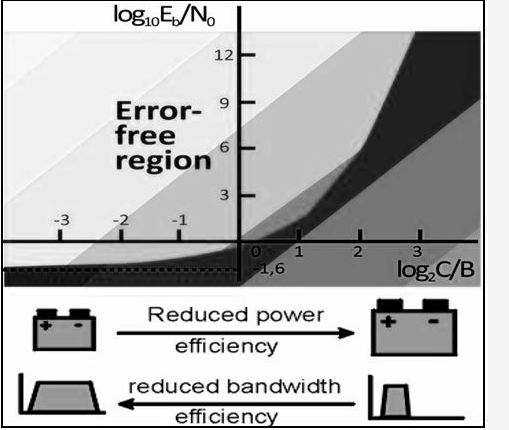
\includegraphics [width=0.75\textwidth]{F/image4.png}
\caption{Shannon–Hartley theorem}
\label{fig:F1}
\end{figure}
 
	The graphical representation of the Shannon–Hartley theorem, see Fig.\ref{fig:F1}, clearly shows that throughput can be traded for power efficiency, and vice-versa. The light gray area represents the area free from errors. The theoretical minimum SNR for an error-free transmission is impossible to reach in practice. The modulation schemes define how close to this theoretical SNRmin the transmission can be. Every modulation scheme is characterized by a minimum SNR that allows the demodulation of the transmitted symbols without errors. Knowing the minimum SNR for every modulation scheme (MS), we can define the minimum Signal Power for every MS for specific levels of noise. The equation that defines the symbol error probability (Ps) for every MS, with respect to SNR is the following \cite{7}:

\begin{equation}
P_{s,M-ary}= (\frac{M-1}{M}) \times erfc(\sqrt{\frac{3}{M^{2}-1} \times \frac{E_{Saver}}{N_{0}}})
\end{equation}

\begin{figure}
\centering
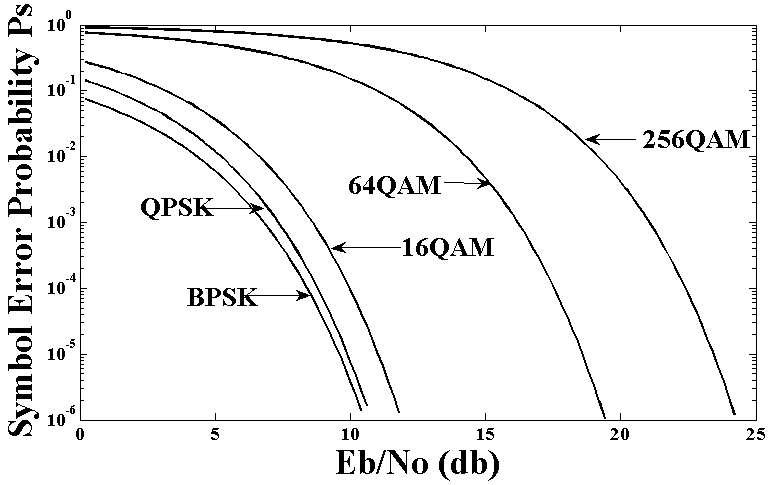
\includegraphics[width=0.75\textwidth]{F/image6.png}
\caption{Symbol error probability for 802.11ac Modulation schemes}
\label{fig:F2}
\end{figure}

\begin{figure}
\centering
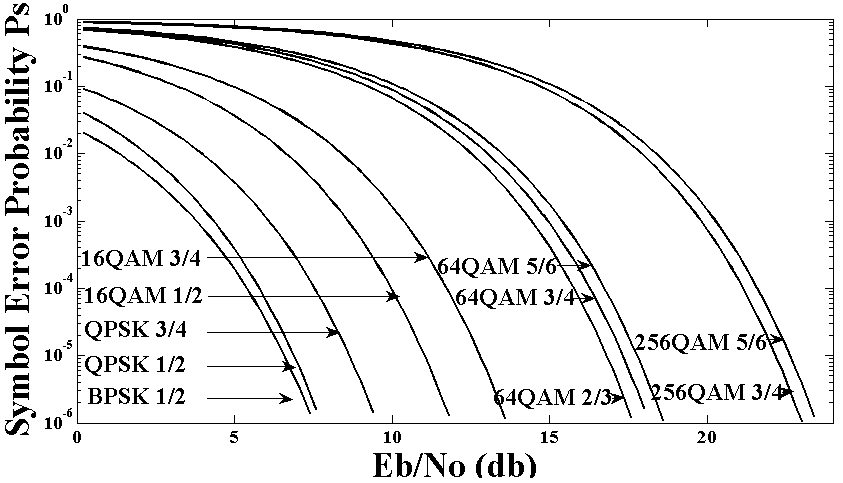
\includegraphics[width=0.75\textwidth]{F/image7.png}
\caption{Symbol error probability for 802.11ac Modulation and Coding schemes}
\label{fig:F3}
\end{figure}

M is the number of symbols used, Es the average received signal power, N0 the average noise signal power and erfc is the complementary error function.
	The graphical expression of this equation for the modulation schemes of the 802.11ac is presented in Fig.\ref{fig:F2}. Channel coding improves the SNR by a factor R \cite{18}. So the curves can be normalized for equal energy per information bit (pre-coding) bearing in mind that the energy per transmitted bit is less than the energy per information bit by a factor equal to the code rate R. The graphical expression of the symbol error probability for the modulation and coding (MC) schemes of the 802.11ac can be found in Fig.\ref{fig:F3}.
	
	In this context, every system scenario RTS is characterized by a two-dimensional cost 1) the total signal power and 2) the bit error rate (BER). The signal power is inversely proportional to the symbol error probability and correspondingly to bit error probability as shown in Fig.\ref{fig:F2} and Fig.\ref{fig:F3}. Each RTS is characterized by a curve in the two-dimensional space of total signal power. This curve is derived by the respective curve at Fig.\ref{fig:F3} that corresponds at the MCs of the RTS. Based on the bits-per-symbol of MCs (BPSK: 1bps, QPSK: 2bps, etc.), the short guard interval (SGI) and the noise level of the RTS, the Ps (symbol error probability) to SNR curve can be transformed to BER to Signal Power curve. In Fig.\ref{fig:F4}, due to limited space, we present 3 representative examples of these RTS curves. For a given BER, the minimum signal power to achieve successful communication is chosen and this point represents the system configuration for this RTS. 
	
\begin{figure}
\centering
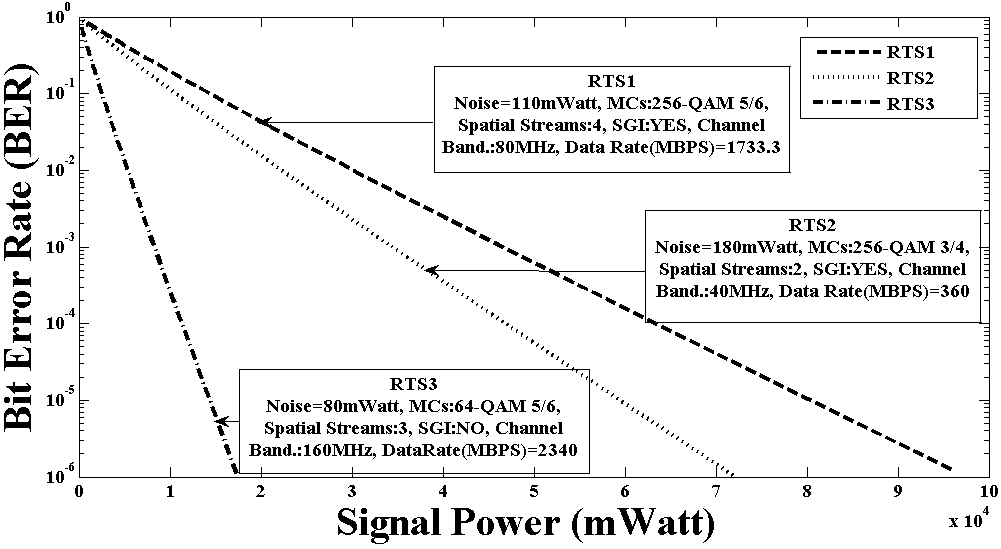
\includegraphics[width=0.75\textwidth]{F/image8.png}
\caption{RTS Characterization}
\label{fig:F4}
\end{figure}	
	
	Besides the above-mentioned technical analysis the most unstable parameter for a transmission is the user profile, e.g., the distance between receiver and transmitter, the existence of other communication channels or others sources of distortion. These are factors that influence the channel transmission and are directly influenced by the user behavior. For example, if the user moves in a saturated spectrum area or in a noisy environment high communication channel interference is expected. Correspondingly, if the user changes position very rapidly, (for example, driving a car) this has impact on the normal demodulation of the transmitted signal (Doppler Effect). 
	
\subsection{Memory Banks}

The SNR level and the changing environment on the wireless channel also affects the memory requirements. In more detail, the conditions of the channel determine the coding and modulation scheme needed for a successful communication and, consequently the required data rate. The coding phase transforms an m-bit data string into an n-bit string in order to be encoded, when the given coding rate is m/n. The modulation phase conveys a varying number of bit streams together, based on the chosen modulation. The data rate constraint defines the storage and transmission requirements for the data. As a result, the memory footprint depends on the data rate of the channel and is dynamic for a changing environment. Energy consumption on the memory subsystem depends on the number of accesses and the energy per access, which are different based on the size and the type of memory.
The observation that the memory requirements at run-time vary significantly due to dynamic variations on the transmission channel and the protocol, is exploited through use of system scenarios. Instead of defining the memory requirements for the worst-case data rate and tuning the system according to this, system scenarios are generated for different situations. The combination of the coding and the modulation parameters define the data rate for each RTS. The data rate is the identification variable and the cost factor is its memory footprint. Based on the cost factor, the different memory footprints are clustered into scenarios. The clustering of RTSs is based both on their distance on the memory size axis and the frequency of their occurrence.

The key feature needed in the platform architecture is the ability to efficiently support different memory sizes that correspond to the system scenarios generated by the methodology. Execution of different system scenarios then leads to different energy costs, as each configuration of the platform results in a specific memory energy consumption. The dynamic memory platform is achieved by organizing the memory area in a varying number of banks that can be switched between different energy states.  

In this work, a clustered memory organization with up to five memory banks of varying sizes is explored. The dynamic memory organization is constructed using commercially available SRAM memory models (MM). For those models delay and energy numbers are derived from a commercial memory compiler. In addition, experimental standard cell-based memories (SCMEM) \cite{19} are considered for smaller memories due to their energy and area efficiency for reasonably small storage capacities. The standard cell-based memories are synthesized using Cadence RTL compiler for TSMC 40nm standard library.

Both MMs and SCMEMs can operate under a wide range of supply voltages, thus support different operating modes that provide an important exploration space. 
\begin{itemize}
\item Active mode: The normal operation mode, in which the memory can be accessed at the maximum supported speed. The supply voltage is 1.1V. The dynamic and leakage power are higher compared to the other modes. In this work all the memory accesses are performed on the active mode.
\item Light/Deep sleep mode: The supply voltage in this mode is lower than active with values around 0.7V and 0.3V respectively. The access time of the memory is significantly higher than the access time in active mode. Switching to active mode can be performed with an energy penalty (switching cost) and a small time penalty of a few clock cycles. Data is retained.
\item Shut down mode: Power-gating techniques are used to achieve near zero leakage power. Stored data is lost. The switch to active mode requires substantially more energy and time. However, switching unused memories to this mode results in substantial energy savings.
\end{itemize}

	The goal is to design a suitable clustered scratchpad memory architecture that can serve the generated scenarios. When the maximum data rate is required by the protocol, all the memory banks should be active and accessed. When the needed data rate is lower, the size and the rate required by the memory system are lower and one or more memory banks can be switched off. As a result, the amount of energy consumed during a system scenario with lower requirements is reduced.
	
\subsection{Combined Model}	

The optimal energy configuration both on the signal power and the memory subsystem takes into consideration six parameters, namely (a) the number of spatial streams (streams), (b) the MC schemes, (c) the channel bandwidth, (d) the SGI, (e) the data rate, and (f) the noise level. Based on their values the run-time manager choses the active scenario for the signal power and the memory subsystem and performs the appropriate reconfigurations. The key point is that this decision is not taken independently. For the first time in the context of a wireless system, two system scenario sets adjusted to achieve an overall optimization. This represents a new methodology extension because the clustering step has to take into consideration not only the overhead impact at the targeted subsystem, but also the interaction with the other subsystem scenario sets. Thus, it is provided an optimal configuration for the whole system and not sub-optimal for individual parts.

\section{Case Study}

In the context of the current case study, we examine the potential power gain exploiting two scenario-based schedulers. The first adjusts dynamically the antenna signal power and the second manages the memory banks activation. For the needs of our study, we consider an artificial application that generates data bursts that have to be transmitted within specific deadlines. The distribution of the generated data bursts is presented at Fig.\ref{fig:F5}. For every data burst there is a corresponding transmission time deadline, which defines a minimum data rate. The distribution of the time deadlines is presented at Fig.\ref{fig:F6}.
 
\begin{figure}
\centering
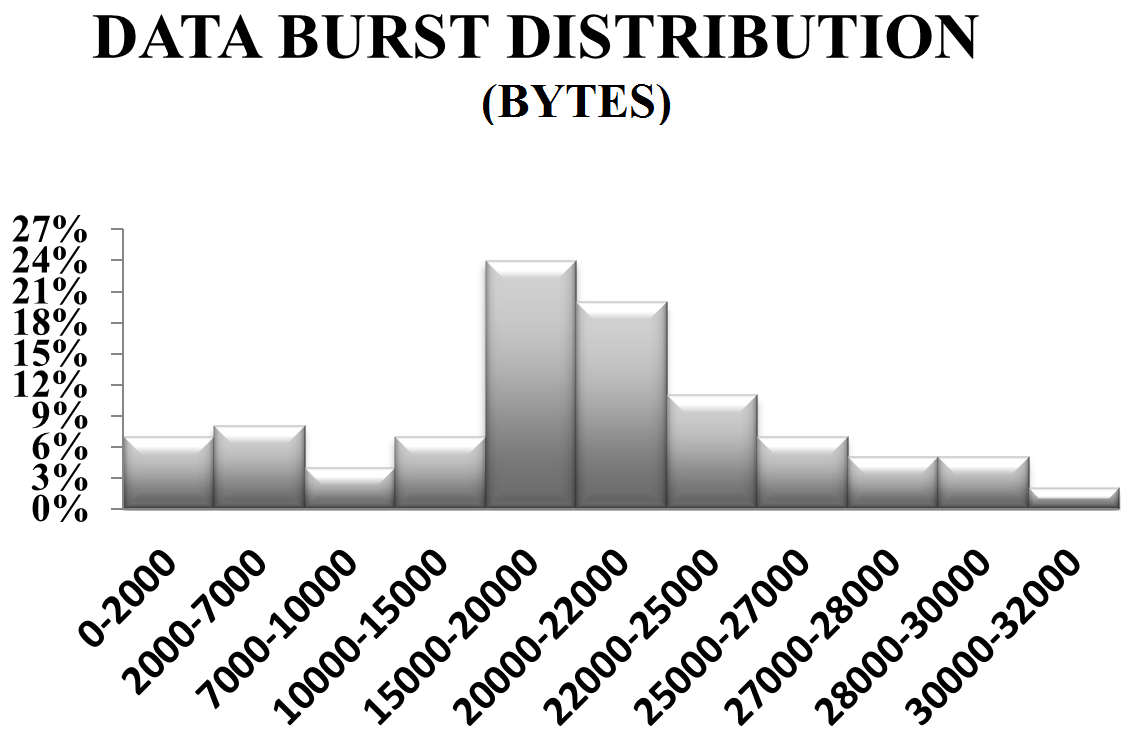
\includegraphics[width=0.75\textwidth]{F/image9.png}
\caption{Data Burst Distribution}
\label{fig:F5}
\end{figure}	

\begin{figure}
\centering
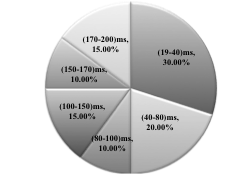
\includegraphics[width=0.75\textwidth]{F/image10.png}
\caption{Application Deadline Distribution}
\label{fig:F6}
\end{figure}	

Every combination of six parameters discussed in Section IV.C represents a different communication scheme. The memory adaptation scheduling takes into consideration only the data rate. The first four parameters (streams, MCs, BW, SGI) is defined by the targeted protocol (802.11ac) \cite{4} creating an exploration space of 240 RTSs. Given values for these four parameters, the maximum value for the fifth parameter, data rate, can be calculated. Thus, data rate does not contribute to the exploration space, but it is used as an identification variable of the suitable communication scheme. More precisely, the desired data rate is extracted dynamically by the running application requirements (Data Bursts size and Deadline) and the scheduler identifies which communication schemes can satisfy this data rate.  
The last and the most important variable is the external noise. In order to be more representative, we take noise distributions and not discrete values of noise.
 For the needs of our measurements we consider two channels with different Gaussian noise distributions as shown in Fig.\ref{fig:F7} having different average values ($\mu$) and standard deviations ($ \sigma $) ($channel_1: \mu  =100mWatt,  \sigma =20mWatt, channel_2:  \mu =140mWatt,  \sigma  = 10mWatt $). 
 The second channel represents a noisier and more rapidly changing environment compared to the first. 
 The noise distribution defines the appearance probability of the running situations (RTSs). 
 A different noise distribution creates a different probability density for the RTSs. For example in our case the probability density of the RTSs, with noise range ($\mu, \mu + \sigma$) and ($\mu$ and $\mu - \sigma$), is 34.13\% (because of the Gaussian distribution). 
 Similarly, the RTSs probability for ($\mu, \mu \pm 2 \sigma$),  ($\mu, \mu \pm 3 \sigma $), ($\mu, \mu \pm 4 \sigma$) and ($\mu, \mu \pm 5 \sigma $) are calculated. 
 Thus, for a Gaussian distribution, we have in total 10 bounding levels of noise, which in combination with the values of the previous parameters creates an exploration space of ($240 \times 10$) 2400 RTSs. The clustering of the RTSs into system scenarios varies based on the noise distributions. Thus, for every distribution we have a different optimal set of system scenarios.

\begin{figure}
\centering
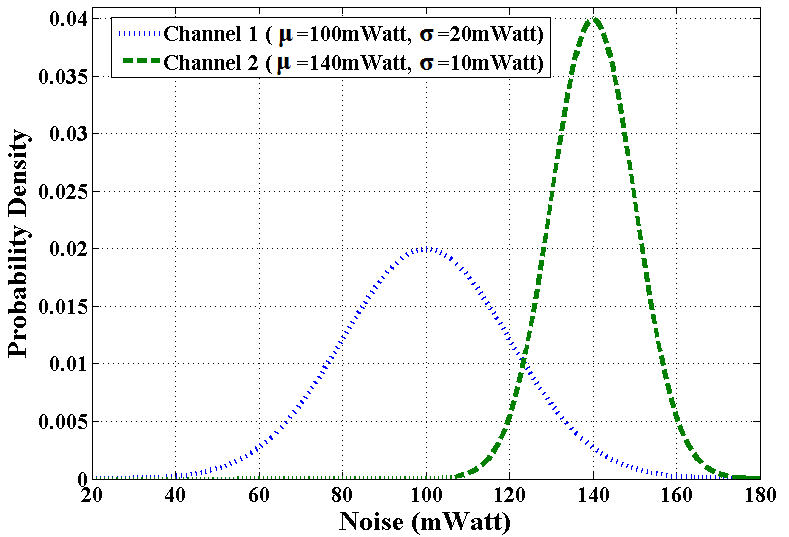
\includegraphics[width=0.75\textwidth]{F/image11.png}
\caption{Noise Distribution}
\label{fig:F7}
\end{figure}	


The scheduling decision about the suitable communication scheme follows three main priorities: 1) the required data rate, 2) the noise tolerance and 3) the power saving. The first criterion fulfills the current application deadlines while the second ensures the signal power for an acceptable BER. Thus, the signal power scheduler first finds the communication schemes that respect the running time constrain, and in a second stage chooses these, that permit the lowest signal power. The final decision is based on the overall system power saving. 

In our case study, we have in total three different sets of system scenarios; two for the signal power scaling (one for each of the two channels presented in Fig.\ref{fig:F7}) and a third set for the memory banks power management (based on the data size distribution presented in Fig.\ref{fig:F5}). To minimize memory bank power, the memory scheduler at run-time activates a suitable number of scratch pad memory banks based on the selected coding scheme. Data are transferred to the memories as part of the transmission chain during the modulation phase.
	
For the extraction of the system scenarios, we take into consideration the trade-off between the run-time implementation overhead and the accuracy of the extracted scenarios. The first is related to the switching overhead while the second is related to the number of the scenarios and the clustering overhead. In comparison with the approach presented in the second case study of publication \cite{21} (related to signal power adaptation), the presented study has the following differentiations. Except from the different characteristics of protocol 802.11ac (compared with 802.11n), in our case the proposed scheduler both adjusts signal power and selects the optimal power communication scheme (MCs, streams, BW etc.) based on the current noise conditions and data rate constrains. This increases the design space complexity from 80 RTSs \cite{21} to 2400 RTSs. Additionally, the current approach takes into consideration two channel noise distributions (one for every channel) which differentiates the RTS appearance frequency, changing dramatically the clustering of RTSs into system scenarios (as the RTS frequency affects significantly the clustering overhead \cite{21}). Furthermore, in the context of the current study we differentiate by presenting the trade-offs between switching and clustering overhead for different numbers of extracted system scenarios and by including memory into exploration. In respect with the last, we insert a new methodology extension adjusting the clustering of two system scenario sets (Signal Power and memory) to achieve an overall optimization.  
	
\section{Results}

	Tab.\ref{tab:F1}, Tab.\ref{tab:F2} and Tab.\ref{tab:F3} present the variation of the clustering and switching overhead. The first column (number of scenarios) gives the number of system scenarios for each row. The second column (clustering overhead compared to WCE) and third column (clustering overhead compared to previous step) presents normalized the percentage variation of the clustering overhead compared with the worst case (monolithic approach) and that of the previous row, respectively. When RTSs are clustered into scenarios, the cost for the most energy demanding RTS is used as the representative cost for all the RTSs within the scenario. The system is configured to serve the most demanding RTS of the scenario and consequently all the less demanding RTSs, which belong to the scenario. The clustering overhead represents the difference between the RTSs within a scenario. As the number of scenarios increases the percentage approaches 100\%, which would be the value if there was a dedicated scenario for each RTS. Similarly, the fourth column (switching overhead) and fifth column (switching var) represents the switching overhead expressed as the scenario switching probability and the percentage change of the switching overhead compared with that of the previous row, respectively.
	
	In Tab.\ref{tab:F1}, for example, for a set of 8 system scenarios we have a clustering overhead of 7\% and a decrease in clustering overhead compared with the previous row (7 system scenarios) of 19\%. The switching overhead is 85\% and it is increased by 4\% compared with the previous row. For an increasing number of scenarios, the clustering overhead is reduced, because the difference between the RTSs within the scenarios decreases. Respectively, the switching overhead is increased, because there are more scenarios to choose from and thus the system switches between scenarios more often. Depending on the design objectives, it is possible to choose an optimized number of scenarios. A larger number of scenarios increases the implementation overhead (more switching overhead) but it reduces the clustering overhead and vice versa.
	
	The power gain percentages for each of the channels and the memory are presented in Fig.\ref{fig:F8}. Results are given for 10 executions of the case study with the noise distribution given in Fig.\ref{fig:F7}. The baseline is a system designed based on the worst-case requirements. The system is assumed monolithic without any reconfiguration based on the noise level and the MC scheme. The gain for the first antenna is around 97\% for all the cases, while for the second antenna it is a little lower. The worst case has a noise level of 180 mWatt, MC scheme 5/6 256QAM, SGI and 4 MIMO, while best case has a noise level of 20 mWatt, MC scheme 1/2 BPSK, no SGI and 1 MIMO. The reported gains for the memory are in the range from 27.8\% to 29\%. The power savings are significantly higher on the antennas due to two main reasons. Firstly, the variation between the best and the worst case on the antennas is wider and thus offers a greater opportunity for energy savings. Secondly, the reconfiguration option for the antennas offer more flexibility and all possible signal power levels can be exploited. The memory architecture has a physical limitation in the number of memories that can be used and only a range of sizes is supported by the system models.

\begin{table}
\centering
	\caption{Memory Banks Scenario Overhead}
	\label{tab:F1}
	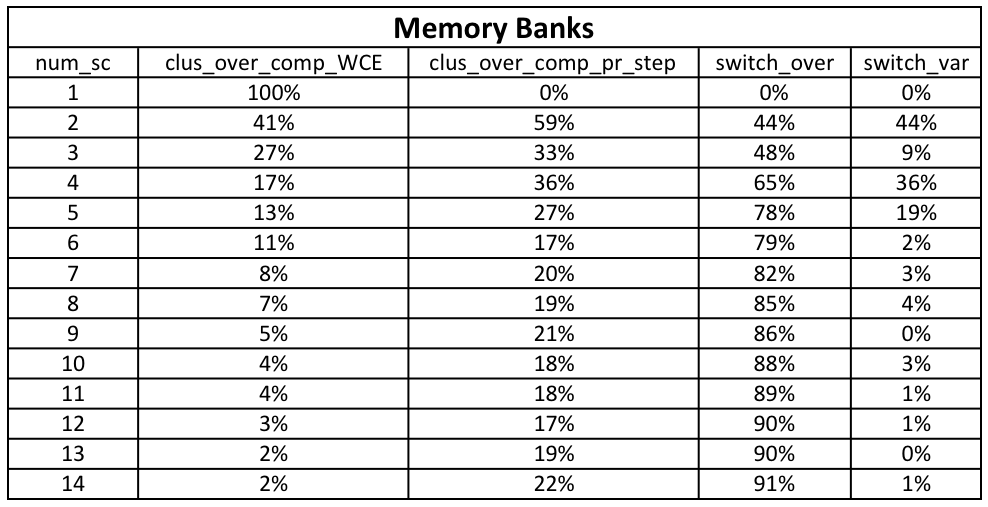
\includegraphics[width=\textwidth]{F/tab1.png}
\end{table} 

\begin{table}
\centering
	\caption{Signal power–Channel 1 Scenario Overhead}
	\label{tab:F2}
	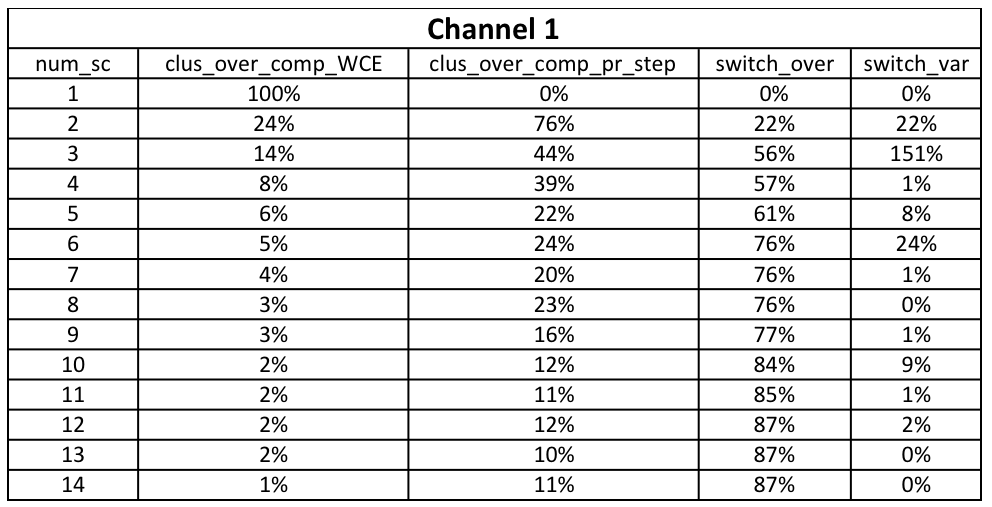
\includegraphics[width=\textwidth]{F/tab2.png}
\end{table} 

\begin{table}
\centering
	\caption{Signal power–Channel 2 Scenario Overhead}
	\label{tab:F3}
	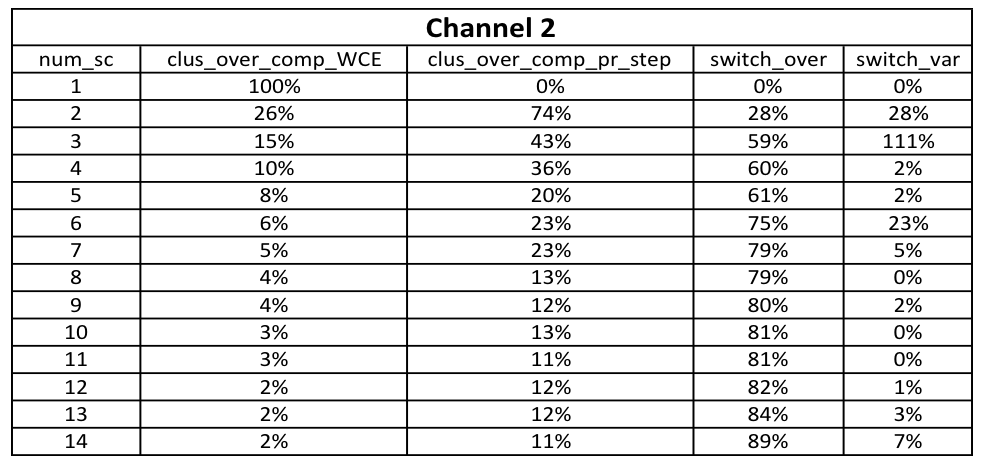
\includegraphics[width=\textwidth]{F/tab3.png}
\end{table} 

\begin{figure}
\centering
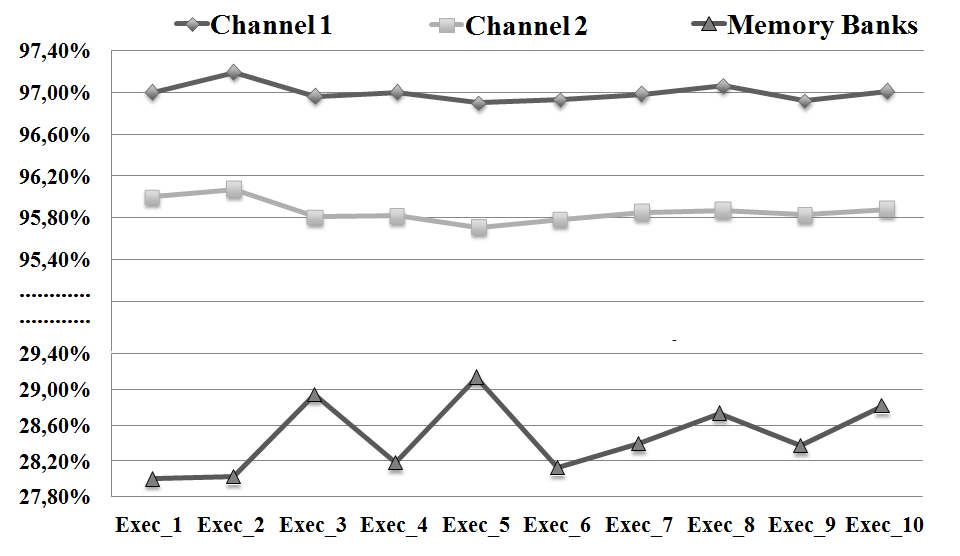
\includegraphics[width=\textwidth]{F/image15.png}
\caption{Power Gain}
\label{fig:F8}
\end{figure}	 

\section{Conclusion} 

The scope of this work is to explore the power management options for a transmitting wireless system using system scenarios. The dynamic parameters and the variations during the transmission for the targeted wireless protocol are analyzed. Based on the analysis and the system models, system scenarios are generated for the case study, in order to optimize energy usage. Both the signal power and the memory subsystem are taken into consideration. The results demonstrate the effectiveness of the methodology and illustrate the interesting trade-off between the clustering overhead and the switching cost. 
	
%\addcontentsline{toc}{section}{Bibliography}	
%\bibliographystyle{plain}
%\bibliography{dsd_ref}
	
	
